\documentclass[11]{article}
\usepackage{amsmath}
\usepackage[in]{fullpage}
\usepackage{tikz}
\usetikzlibrary{er}
\usetikzlibrary{positioning,shapes,shadows,arrows}
\newcommand{\HRule}{\rule{\linewidth}{0.3mm}}
\usepackage{multicol}
\usepackage{lipsum}% dummy text
\usepackage{tikz}
\def\checkmark{\tikz\fill[scale=0.4](0,.35) -- (.25,0) -- (1,.7) -- (.25,.15) -- cycle;} 
\setlength{\columnseprule}{0.4pt}
\begin{document}
\centerline{\Large \textsc{ \textbf{Home Management System}}} \smallskip
\centerline{\large \textsc{ \textbf{Project Proposal}}} \smallskip
\noindent\HRule \\
\ \\
\textbf{Description} \\
Home management portal to track home related activity such as expenses, grocery purchases, who is cooking next, whose turn is in cleaning trash using a combination of functions like expense manager, to do list, note taking utilities along with a instant messenger for member communication regarding the activity. \\
\ \\
\noindent \textbf{Users} \\
Each project(name for new profile) consists of groups. Group can be created by one or more individual members. The portal consists of three abstract activity.  \\
\ \\
\noindent \textbf{Activity} \\
Task, List and Expense. Task involves work which will consume time of the activity based on the type of work, example Trash cleaning or cooking. List is a way to specify items in a order or unordered form, grocery listing for next week or things to repair in house. Expense activity will involve the money component in it, grocery purchases, refueling vechile. One or more combination can be used to create groups. The groups will encompass members. The task alone group will be cooking turns. Expense activity will involve trips. List activity will involve. Below is the example of each.\\

\begin{minipage}{0.32\textwidth}

\end{minipage}%
\hfill
\begin{minipage}{0.32\textwidth}
\begin{tabular}{|p{\textwidth}}

\end{tabular}
\end{minipage}%
\hfill
\begin{minipage}{0.32\textwidth}
\begin{tabular}{|p{\textwidth}}

\end{tabular}
\end{minipage}%

\begin{table}[h] % http://en.wikibooks.org/wiki/LaTeX/Tables
\begin{center}
\caption{Task }
	\begin{tabular}{| c | c |} % number of c's is the number of columns; options are r, l, c (that's a lowercase L). I also use a vertical pipe (|) for vertical lines in the table. This can get really confusing, since l (L) and | (pipe) look identical. Leave the pipes out of your default code.
	\hline
	Cooking & \checkmark \\  % put & between columns
	\hline
	Bob & \checkmark \\  % put & between columns
	\hline
		Ram & \checkmark \\  % put & between columns
	\hline
		Jay & \checkmark \\  % put & between columns
	\hline
		Diya & \checkmark \\  % put & between columns
	\hline
		Robert &  \\  % put & between columns
	\hline
		Linda &  \\  % put & between columns
	\hline
		John &  \\  % put & between columns
	\hline
	\end{tabular}
\end{center}
\end{table}


\begin{table}[h] % http://en.wikibooks.org/wiki/LaTeX/Tables
\begin{center}
\caption{Listing }
	\begin{tabular}{| c | c | c |} % number of c's is the number of columns; options are r, l, c (that's a lowercase L). I also use a vertical pipe (|) for vertical lines in the table. This can get really confusing, since l (L) and | (pipe) look identical. Leave the pipes out of your default code.
	\hline
	Cooking & Qty & \checkmark \\  % put & between columns
	\hline
	Rice & 10 kg & \checkmark \\  % put & between columns
	\hline
		Wheat Flour & 10 kg &  \\  % put & between columns
	\hline
		Tortilla & 10 pc & \\  % put & between columns
	\hline
		Milk & 3 Gallons & \\  % put & between columns
	\hline
		Eggs &  18 & \\  % put & between columns
	\hline
	\end{tabular}
\end{center}
\end{table}

\begin{table}[h] % http://en.wikibooks.org/wiki/LaTeX/Tables
\begin{center}
\caption{Expense }
	\begin{tabular}{| l | l | c |} % number of c's is the number of columns; options are r, l, c (that's a lowercase L). I also use a vertical pipe (|) for vertical lines in the table. This can get really confusing, since l (L) and | (pipe) look identical. Leave the pipes out of your default code.
	\hline
	Item & Cost & Paid by \\  % put & between columns
	\hline
	Rice & \$20 & Ram \\  % put & between columns
	\hline
		Wheat Flour & \$20 & Diya \\  % put & between columns
	\hline
		Tortilla & \$5 & John \\  % put & between columns
	\hline
		Milk & \$2.5 & \\  % put & between columns
	\hline
		Eggs &  \$4 & \\  % put & between columns
	\hline
	\end{tabular}
\end{center}
\end{table}
\ \\
\noindent \textbf{Scope} \\
Each users in the given project will have equal access. The groups can be created with the registered members or non-registered members. Registered members can create new groups, add, delete or modify items. Non-registered members can add, delete or modify items. Non-registered members entry will be added into Members with partial access.
\ \\
\noindent \textbf{Tables} \\
Members(\underline{MemberID},MemberName,Email,Phone) \\
Groups(\underline{GroupID,MemberID},GroupName) \\
Expenses(\underline{TransactionID},GroupID,MemberID,TransactionItem,Cost,ShareType) \\
Listing(\underline{ListingID},GroupID,MemberID,List,Status) \\
Task(\underline{TaskID},GroupID,MemberID,Task,Status) \\
InstantMessage(\underline{MessageID},ToID,FromID,Message,Time,Privacy,tags) \\
\ \\
\noindent \textbf{Entity Relationship Diagram} \\
{\color{red}Incomplete }
\iffalse \tikzstyle{every attribute} = [top color=white, node distance=2.5cm]
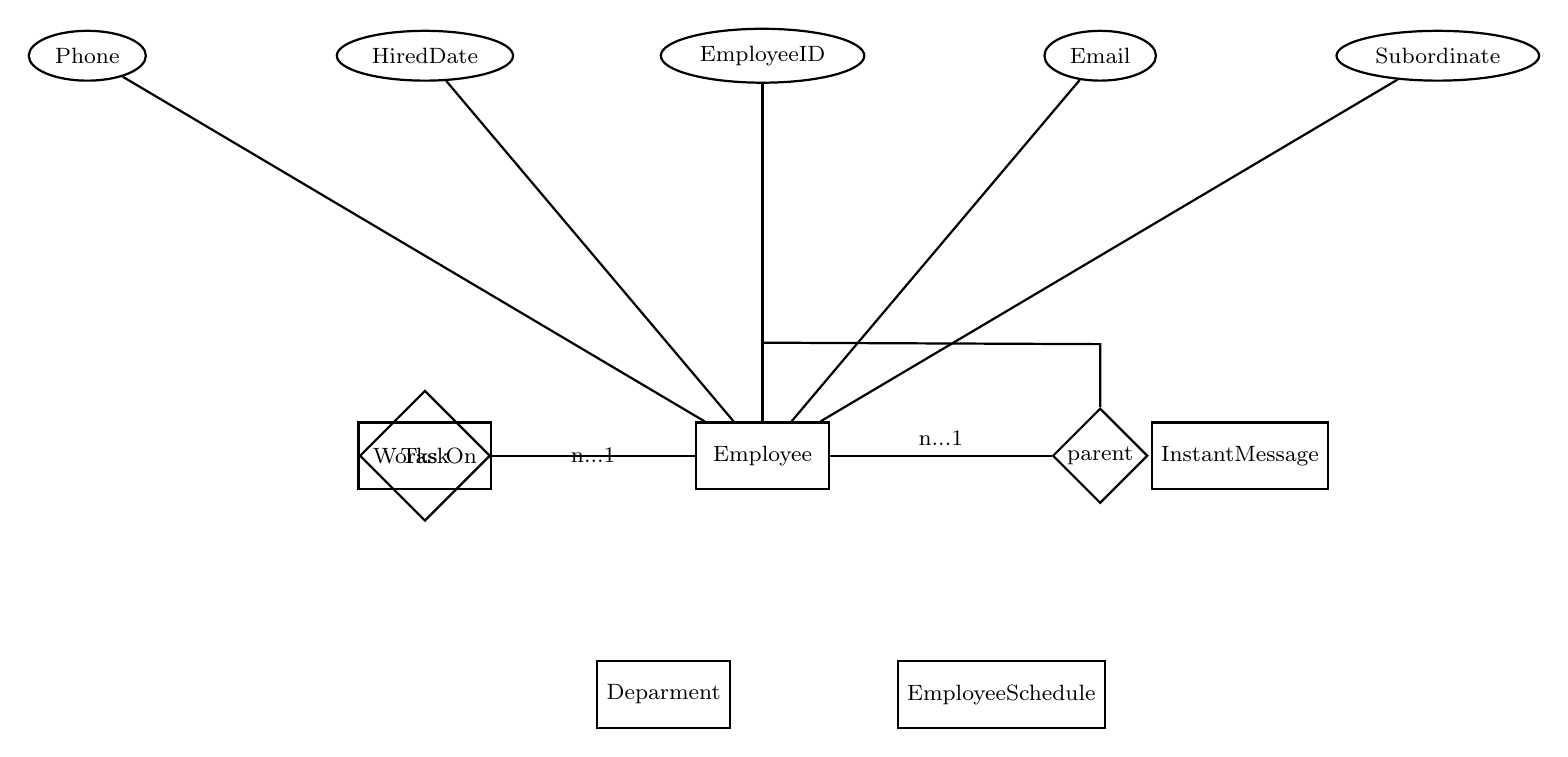
\begin{tikzpicture}[>=open triangle 90, thick,every node/.style={font=\footnotesize}, node distance = 12.2em]
\node[entity](Employee){Employee};
\node[attribute] (eid) [above=of Employee] {EmployeeID} edge (Employee);
\node[attribute] (hdate) [left of=eid] {HiredDate} edge (Employee);
\node[attribute] (email) [right of=eid] {Email} edge (Employee);
\node[attribute] (phone) [left of=hdate] {Phone} edge (Employee);
\node[attribute] (subordinate) [right of=email] {Subordinate} edge (Employee);

\node[entity](Task)[left of =Employee]{Task};

\node[entity](Deparment)[below right of =Task]{Deparment};

\node[entity](EmployeeSchedule)[right of =Deparment]{EmployeeSchedule};

\node[entity](InstantMessage)[above right of =EmployeeSchedule]{InstantMessage};

\node[relationship] (pageparent) [right of =Employee] {parent} edge node[above]{n...1} (Employee) edge (Employee);
\node[relationship] (EmployeeTask) [left of =Employee] {Works On} edge node {n...1} (Employee) edge (Task);
\coordinate[above= 1cm of Employee] (cpage);
\coordinate[above= 0.8cm of pageparent] (cpageparent);
\draw[-] (Employee)--(cpage)--(cpageparent)--(pageparent);
\end{tikzpicture}
\fi
\ \\
\noindent \textbf{Implementation} \\
Database implementation is using PostgreSQL and MongoDB(Messaging table alone). User interface is either using html/php or AngularJS.
\end{document}